%%%%%%%%%%%%%%%%%%%%%%%%%%%%%%%%%%%%%%%%%
% Short Sectioned Assignment
% LaTeX Template
% Version 1.0 (5/5/12)
%
% This template has been downloaded from:
% http://www.LaTeXTemplates.com
%
% Original author:
% Frits Wenneker (http://www.howtotex.com)
%
% License:
% CC BY-NC-SA 3.0 (http://creativecommons.org/licenses/by-nc-sa/3.0/)
%
%%%%%%%%%%%%%%%%%%%%%%%%%%%%%%%%%%%%%%%%%

%----------------------------------------------------------------------------------------
%	PACKAGES AND OTHER DOCUMENT CONFIGURATIONS
%----------------------------------------------------------------------------------------

\documentclass[paper=a4, fontsize=11pt]{scrartcl} % A4 paper and 11pt font size

\usepackage[T1]{fontenc} % Use 8-bit encoding that has 256 glyphs
\usepackage{fourier} % Use the Adobe Utopia font for the document - comment this line to return to the LaTeX default
\usepackage[english]{babel} % English language/hyphenation
\usepackage{amsmath,amsfonts,amsthm} % Math packages

\usepackage{lipsum} % Used for inserting dummy 'Lorem ipsum' text into the template

\usepackage{sectsty} % Allows customizing section commands
\allsectionsfont{\centering \normalfont\scshape} % Make all sections centered, the default font and small caps

\usepackage{fancyhdr} % Custom headers and footers
\pagestyle{fancyplain} % Makes all pages in the document conform to the custom headers and footers
\fancyhead{} % No page header - if you want one, create it in the same way as the footers below
\fancyfoot[L]{} % Empty left footer
\fancyfoot[C]{} % Empty center footer
\fancyfoot[R]{\thepage} % Page numbering for right footer
\renewcommand{\headrulewidth}{0pt} % Remove header underlines
\renewcommand{\footrulewidth}{0pt} % Remove footer underlines
\setlength{\headheight}{13.6pt} % Customize the height of the header

\numberwithin{equation}{section} % Number equations within sections (i.e. 1.1, 1.2, 2.1, 2.2 instead of 1, 2, 3, 4)
\numberwithin{figure}{section} % Number figures within sections (i.e. 1.1, 1.2, 2.1, 2.2 instead of 1, 2, 3, 4)
\numberwithin{table}{section} % Number tables within sections (i.e. 1.1, 1.2, 2.1, 2.2 instead of 1, 2, 3, 4)

\setlength\parindent{0pt} % Removes all indentation from paragraphs - comment this line for an assignment with lots of text

\usepackage{graphicx}

%----------------------------------------------------------------------------------------
%	TITLE SECTION
%----------------------------------------------------------------------------------------

\newcommand{\horrule}[1]{\rule{\linewidth}{#1}} % Create horizontal rule command with 1 argument of height

\title{	
\normalfont \normalsize 
\textsc{University of California San Diego} \\ [25pt] % Your university, school and/or department name(s)
\horrule{0.5pt} \\[0.4cm] % Thin top horizontal rule
\huge CSE 260 -- Parallel Computation \\ Programming Lab 1 \\ High Performance Matrix Multiplication \\ Group ID: G-418-960 % The assignment title
\horrule{2pt} \\[0.5cm] % Thick bottom horizontal rule
}

\author{Andreas Prodromou, Samuel Wasmundt \\ <A530-492-30>, <A530-537-28>} % Your name

\date{\normalsize\today} % Today's date or a custom date

\begin{document}

\maketitle % Print the title

%----------------------------------------------------------------------------------------
%	PROBLEM 1
%----------------------------------------------------------------------------------------

\section{\textbf{High Performance Matrix Multiplication}}

Matrix multiplication is a very common function amongst applications that require high-performance. Various performance improvements were suggested in the past and implemented in the ATLAS library. The goal of this assignment was to optimize matrix multiplication performance on a single core. This report describes the various optimizations implemented by our group and the impact of these optimizations in terms of GFlops/s.\\

The starter code provided was a matrix multiplication implementation with one level of blocking to improve performance over the ``naive'' implementation that simply traverses the matrices in order and performs multiplications and additions to compute the final result.\\

Our group extended the starter source code with a second level of cache blocking and a combination of other performance optimizations such as loop unrolling, array alignment, write combining, and the use of SSE intrinsic commands. SSE commands proved to play a vital role in improving the single-core performance by utilizing the core's SIMD capabilities.\\

The following sections provide some details over the implemented optimizations, along with some background details explaining why each method improves the performance. Results are presented in the form graphs to visualize the optimizations' impact.

\section{\textbf{Cache Blocking}}

As described in the introductory section, the starter code provided us with an algorithm that performs one level of cache blocking on the input matrices and performs the multiplications. Compared to the naive implementation we observe a noticable improvement, especially when multiplying large matrices.\\

The term ``blocking'' implies that the input matrices are divided into smaller ``sub-blocks'' and then these sub-blocks are multiplied with each other in a combination which assures that all the required multiplications took place. The reason for the observed performance improvement relies deep in the core's microarchitecture. During a large matrix multiplication, the core's cache cannot hold all the required memory to support the software's logic. This results in an increasing number of cache-misses, which consequently lead to a major performance hit. As expected, the size of the sub-blocks is another important decision that affects performance. Large sub-blocks might still not fit in the cache, while small sub-blocks do not utilize the cache efficiently.

\begin{figure}[h]
  \centering
    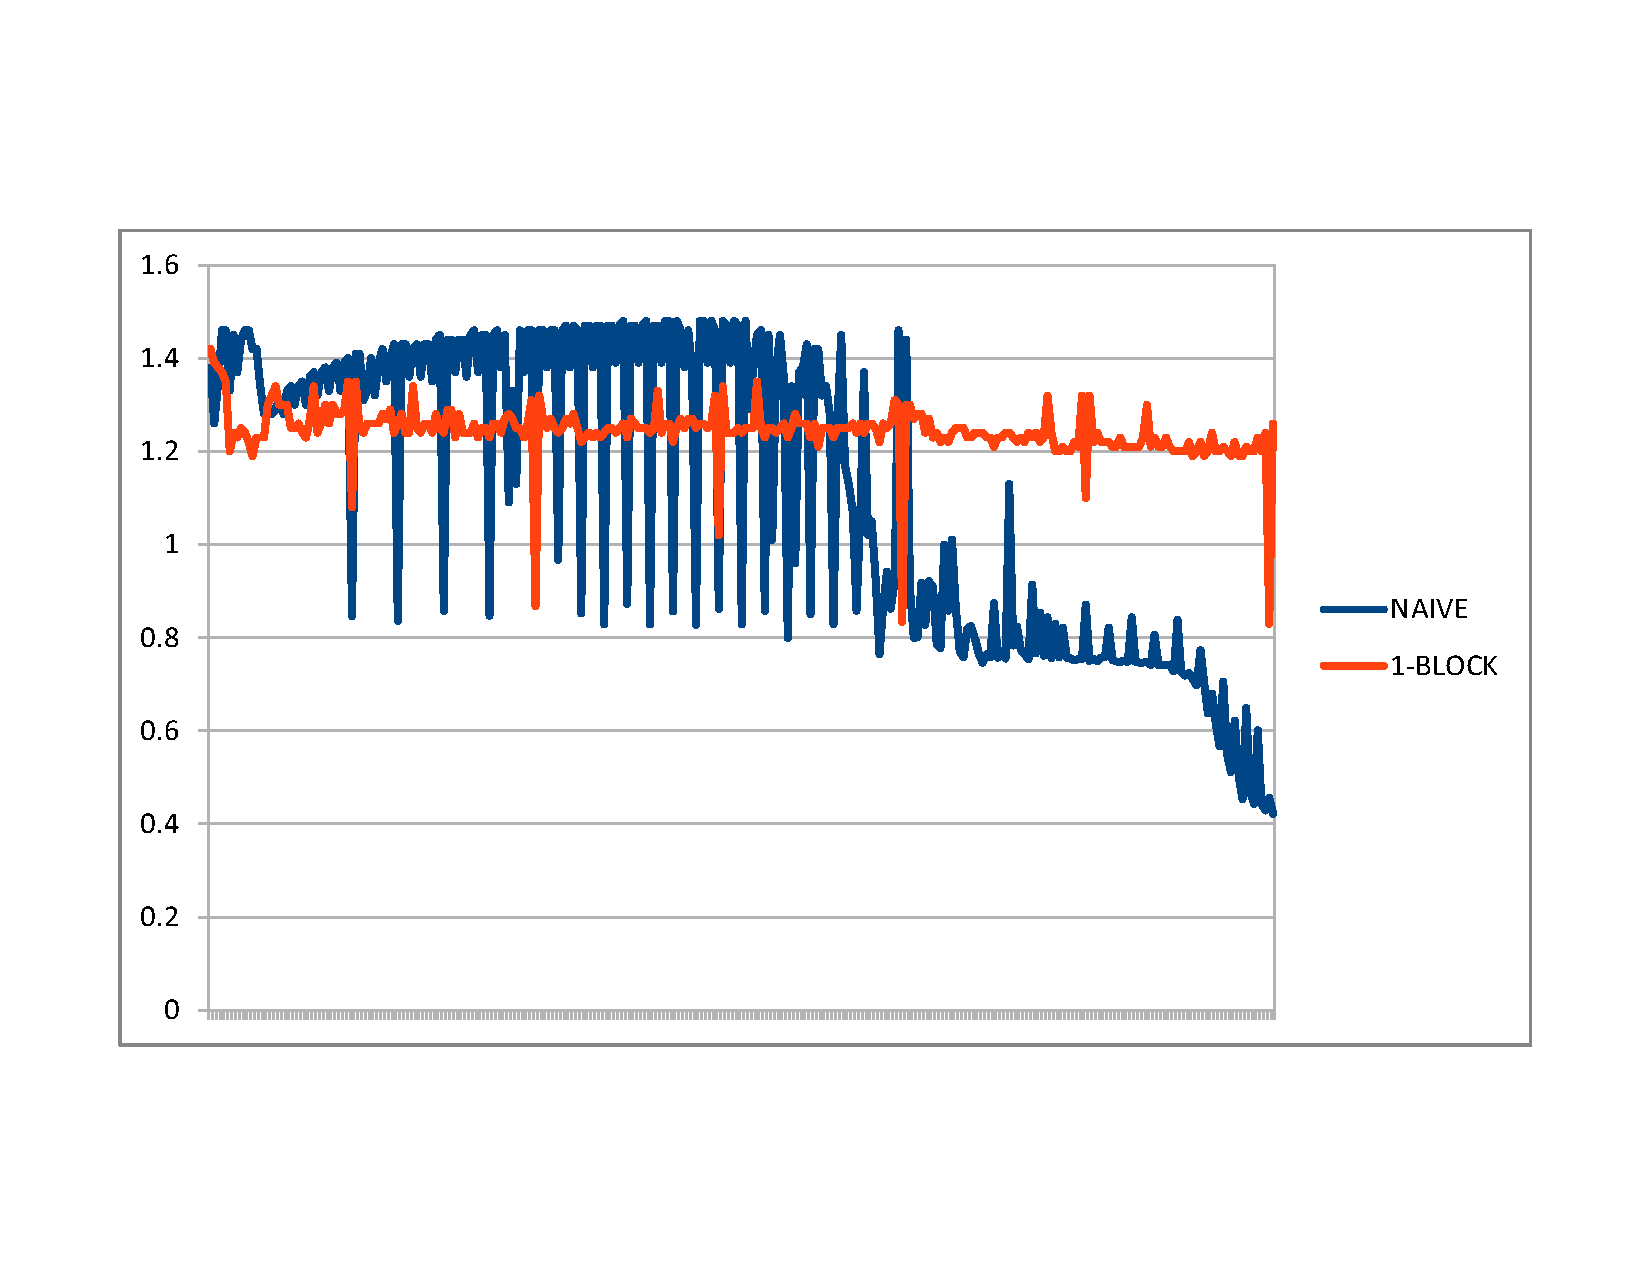
\includegraphics[width=0.8\textwidth]{figures/one_block.pdf}
    \caption{Performance with Single Blocking Level}
    \label{fig:one_blocking_level}
\end{figure}

Dividing large matrices into sub-blocks requires more effort by the programmer, however it significantly increases the number of cache-hits by utilizing locality within the code. The downside to this is that often times the cache characteristics will vary from machine to machine, and as a result fine tuning will need to be done on the end machine. Figure \ref{fig:one_blocking_level} displays the performance improvement after one level of blocking over the ``naive'' code.



\subsection{\textbf{Second Level of Cache Blocking}}

Along the lines of the given performance optimization, we implemented a second level of cache blocking. Following the same logic, we want the first division into sub-blocks to hold as much data as possible in the L2 cache and then we further divide the sub-blocks into smaller chunks that fit in the L1 cache. This way we utilize all the cache levels of our core as much as possible.\\

Since this optimization is essentially a recursive call over the first optimization, our source code is essentially performing the exact same steps as the first blocking level with the only difference being that it now performs blocking on a different-sized matrix. Figure \ref{fig:second_blocking_level} demonstrates the prformance increase obtained by implementing a second level of cache blocking in comparison to the naive approach and the single-blocking level optimization.

\begin{figure}[h]
  \centering
    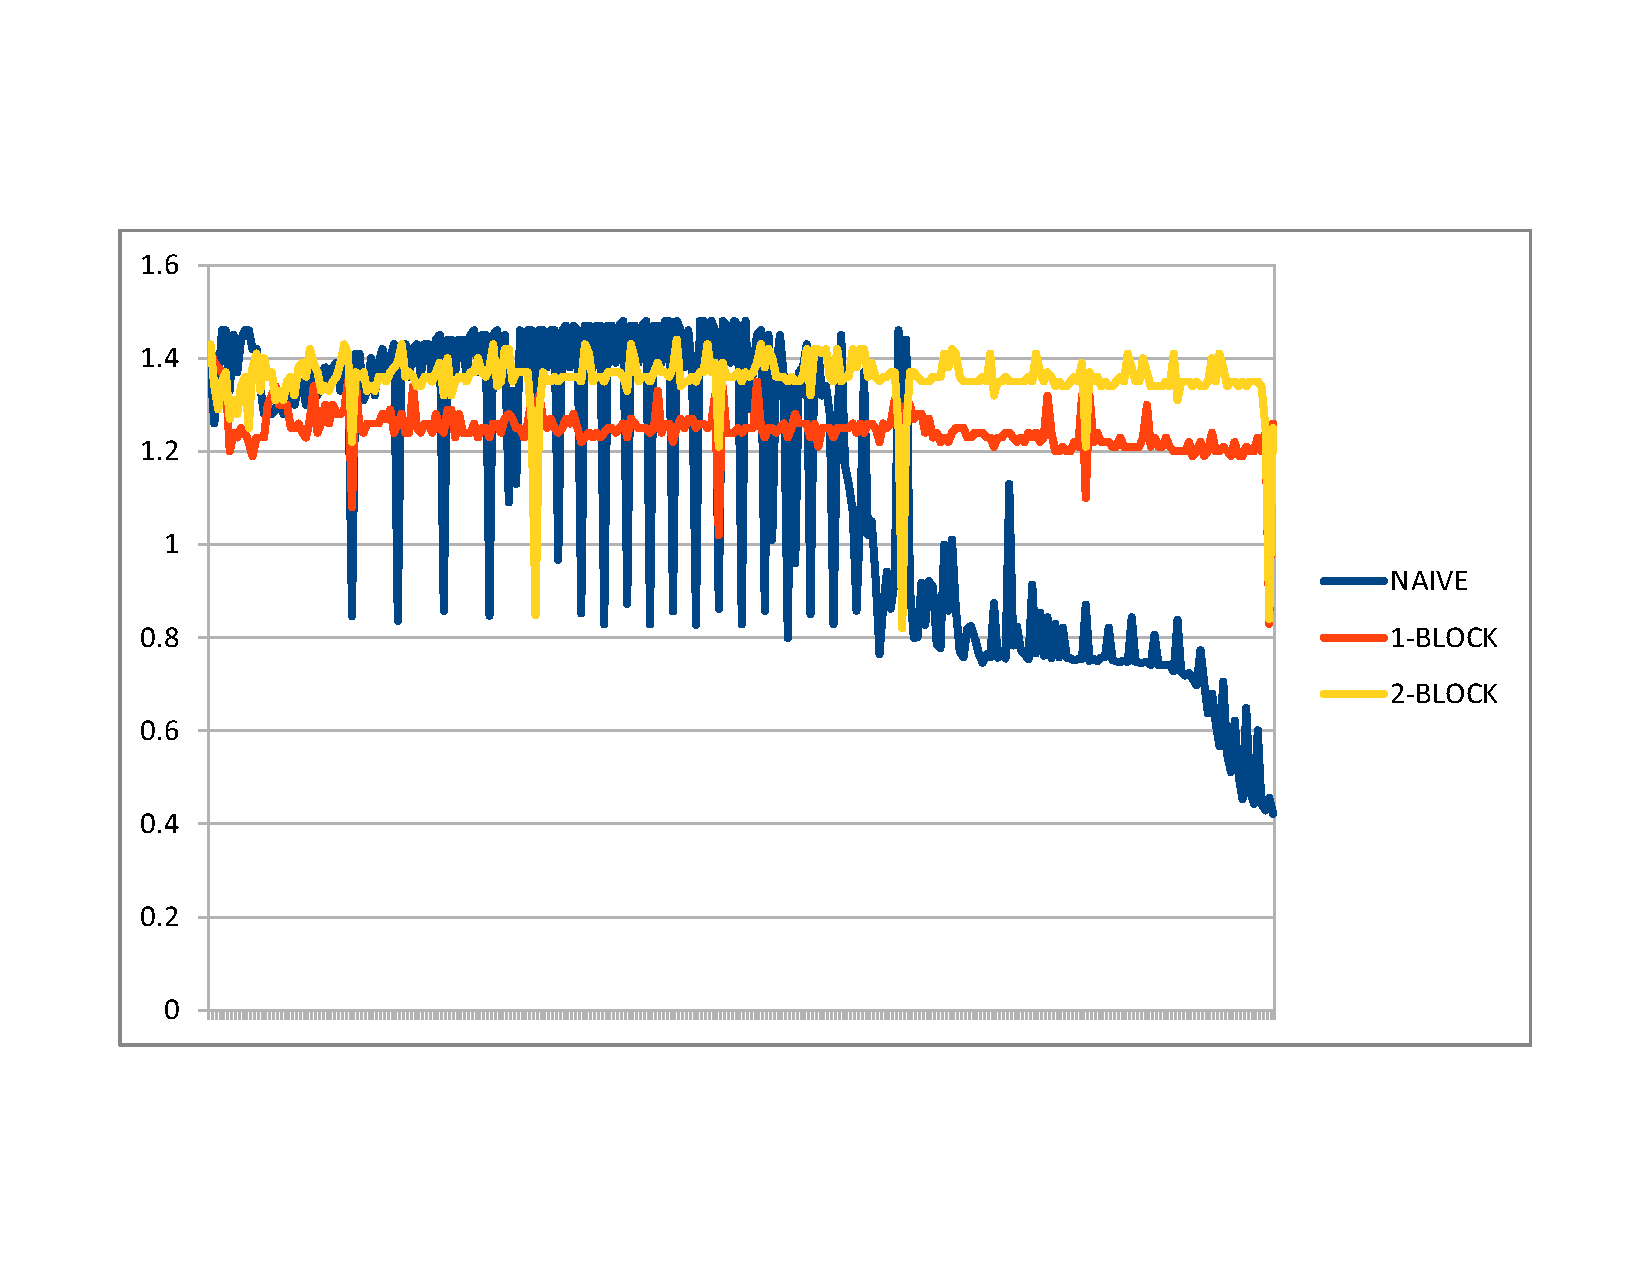
\includegraphics[width=0.8\textwidth]{figures/two_blocks.pdf}
    \caption{Performance with Two Blocking Levels}
    \label{fig:second_blocking_level}
\end{figure}

\subsection{\textbf{Optimal Cache Blocking Sizes}}

As described earlier, we need to determine the sizes for the two levels of cache blocking in such a way that our program utilizes the two levels of cache efficiently (i.e. Fill the caches as much as possible without exceeding their capacities). To determine these numbers, we need knowledge of the processor's cache sizes.\\

In our case, the processor used is an Intel Xeon 5345 with 32KB of L1 cache and 4MB of L2 cache. We begin with determining the optimal sub-block size for the first blocking level. Since this level will position blocks of memory in the L2 cache, we have to figure out a number (BLOCK\_SIZE\_1) such as the L2 cache is filled as much as possible by holding three sub-blocks (A, B and C, where C = A * B). So knowing that we have an L2 of 4MB we calculate we will have $\sqrt{4MB/8/3} = 209$ entries for each A, B, and C. Likewise, for the L1 cache, which is 32KB, we have $\sqrt{32KB/8/3} = 36$. As an optimization to handle the boundary cases as described below, we made temporary variables A*, B*, and C* subject them to being a multiple of 4. Thus, the final sizes we decided on were 192 for BLOCK\_SIZE\_1 and 32 for BLOCK\_SIZE\_2.

\subsection{\textbf{Handling the Boundary Cases}}
A significant effort was put into handling matrix multiplication with any given M, N, and K for any BLOCK\_SIZE\_1 and BLOCK\_SIZE\_2 parameters. For performance, we were able to implement a matrix multiplication that could correctly handle any combination of these without the use of any if conditionals. The initial matrix multiplication performed as many 4x4 SSE matrix multiplications (more on this in the next section) and followed up by performing the proper amount of 'cleanup' multiplications that were unable to be performed by doing 4x4 multiplication blocks. We were able to directly improve upon this performance by actually simplifying the matrix multiplication. Instead of directly handling the boundary cases, we simply take the inputed arrays of A, B, and C and create new temporary arrays A*, B*, and C* that have been padded with 0's to allow for a perfect division into BLOCK\_SIZE\_1, which further by design can be broken exactly into BLOCK\_SIZE\_2 sized chunks. Thus, we know that the A*, B*, and C* matrices being passed to our matrix multiplication will always be divisible by 4! By padding the input A, B, and C arrays with 0's we are able to perform 4x4 block matrix multiplications without worrying about erroniously computing C. Further, these arrays are now aligned arrays which also improves performance.

\section{\textbf{SIMD Optimization -- SSE Instructions}}
Bang has support for 16x128 bit SSE3 registers. Since we are opperating on doubles, each variable uses 64 bits of space. This effectively gives us 32 usable double precision registers. Taking this into account, we expanded upon the 2x2 SSE Matrix Multiplication provided by Professor Baden in lecture and perform a 4x4 SSE Matrix Multiplication. This requires us to use 16 double precision registers to load and store our result, 4 to load in A, and 4 to load B, for a total of 24 double precision values. Note that the 4 values of A are forming a matrix column, and as such they have to be loaded into different registers. As a consequence, our program utilizes a total of 14 XMM registers. By replacing a naive matrix multiplication that does a simple dot product of each row and collum of A and B, respectively, and stores the result in C with the SSE intrinsics instructions we were able to see a speedup.\\ 

In an attempt to improve performance we tried several different configurations of the SSE matrix multiplication. Initially, we had a 2x2 SSE matrix multiplication implemented and contrasted this with that of a 4x4. Due to the underlying hardware on Bang, the 4x4 won out. More concretely, with a 2x2 SSE multiplication being performed it was not enough to adequately saturate the 16x128 bit registers provided by Bang. By bumping up the matrix multiplication to a 4x4, we were able to fully utilize the resources. One thing that we did not experiment with, due to time constraints, was performing multiplication on matrices such as 2x4, 3x4, 4x2, etc. Theoretically one of these could have outperformed our 4x4 is if there was an unforseen register contention.\\

Figure \ref{fig:sse} demonstrates the speedup achieved by utilizing the processor's SIMD capabilitites. Some discussion is required to provide a better understanding of this figure. The line SSE-192 demonstrates exactly what we described up to this point in this document. BLOCK\_SIZE\_1 was set to 192 for the reasons described earlier and SSE intrinsics were used. We observe high spikes in our graph (higher than the SSE-16 case) however we also observe periods of very low performance. On the other hand, SSE-16 (BLOCK\_SIZE\_1 was set to 16) shows lower peak performance, however very few periods of bad performance compared to SSE-192. The reason for the observed behavior is the alignment of the arrays and padding them with 0's. When the block size is relatively small, less memory locations need to be padded with 0 and as a side-effect less calculations need to be performed. For example, with a block size of 192, an array of size 193$\times$193 would be reshaped into an array of size 384$\times$384 with the extra space being set to zero. With a small block size, the impact of alignment and padding is minimal.

\begin{figure}[h]
  \centering
    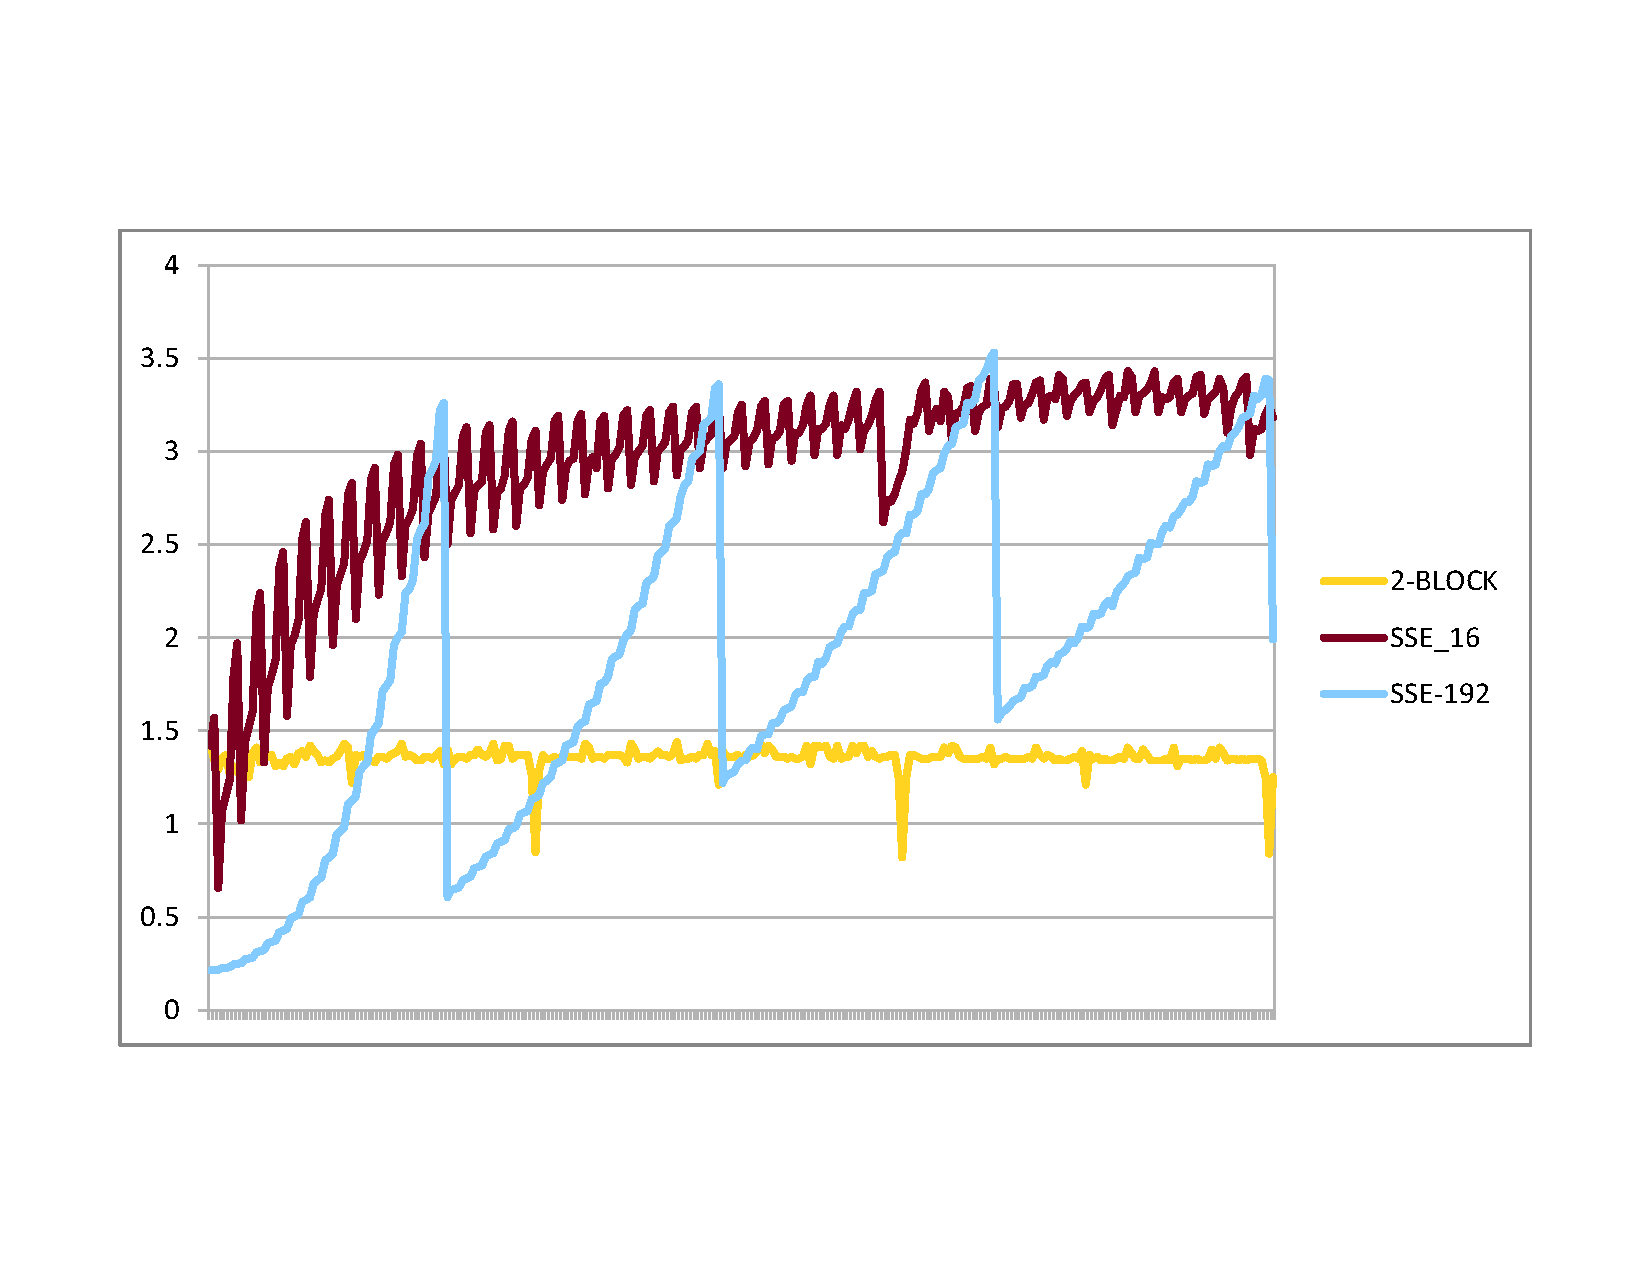
\includegraphics[width=0.8\textwidth]{figures/sse.pdf}
    \caption{Performance using SSE Intrinsics}
    \label{fig:sse}
\end{figure}

\section{\textbf{Other Optimizations}}
Some of the other optimizations we looked into were transposing B to generate better cache locality, creating temporary arrays to align memory as discussed above, and write combining. Optimizations that weren't fully explored due to time constraints were optimizing TLB misses and exploring with SSE matrix multiplication dimensions. We also attempted loop unrolling within the SSE matrix multiplication portion.

\subsection{\textbf{Matrix Transposition}} 
This proved not to be that beneficial to use because we had already created our temporary B* array that allowed us to load aligned blocks. Though we were able to get an entire line of A, and an entire collumn of B (which corresponds to an entire row of B*), we were unable to effectively use them in an SSE supported way that gained us performance benefits. This is due to the fact that we needed shift operation to get the data where it needed to be able to perform the operations supported by SSE in order to get the correct result matrix.

\subsection{\textbf{Aligned Temporary Arrays}}
As discussed earlier, by creating temporary storage arrays A*, B*, and C* that were aligned we were able to see performance increases. A specific thing to note about this is that we saw our performance increase from this optimization as the size of the array being operated on grew. This is because the memory is an $O(N^2)$ operation, whereas the computation of the matrix multiplication is $O(N^3)$. Thus, as the size of our arrays grow, this performance optimizations plays a bigger and bigger role. 

\subsection{\textbf{Write Combining}}
This was a simple two fold optimization. Instead of performing multiple writes to one memory location, we created a temporary variable that we updated and only updated the memory location after all local computation was complete. Further, we tried combining these writes whenever possible to utilize write bandwidth. An example of write combining is when we are creating our temporary A*, B*, and C* arrays we do not create them all within one loop, instead we do them in 3 separate loops that allows each to be combined, utilizing the write/read bandwidth of memory. Essentially eliminating a bottleneck that would occur if we need to access 3 different parts of memory for A, B, and C during each iteration. This way we are able to grab larger chunks at a time. Theoretically this is simple enough that the compiler should be able to handle it, but in our analysis we saw improvements having the loops broken apart.

\subsection{\textbf{Loop Unrolling}}
One last optimization that we attempted was to try unrolling the for loop within our SSE matrix multiplication. In doing so we didn't have a need for any more C registers, as the C matrix was fully represented already, we did however need to add 4 more A and B registers which brought the total register consumption to 16. After a performance analysis, it was shown to be detrimental to unroll the for loop. We speculate the reason for this to be due to register contention.

\section{\textbf{Verification}}
We found the checking mechanism within the benchmark driver to be insufficient to detect all errors within our matrix multiplication. We implemented a self checking method that would fully check the returned C value with what was expected, erroring when an incorrect result was returned. This proved to be very beneficial as we were modifying out code.\\

\section{\textbf{Conclusions}}
This report presents all the optimizations that were performed by our group in an attempt to optimize matrix multiplication as much as possible. Not all the optimizations described are part of the final program, since in some cases certain optimizations ended up hurting performance in the presence of other optimizations.\\

\begin{figure}[h]
  \centering
    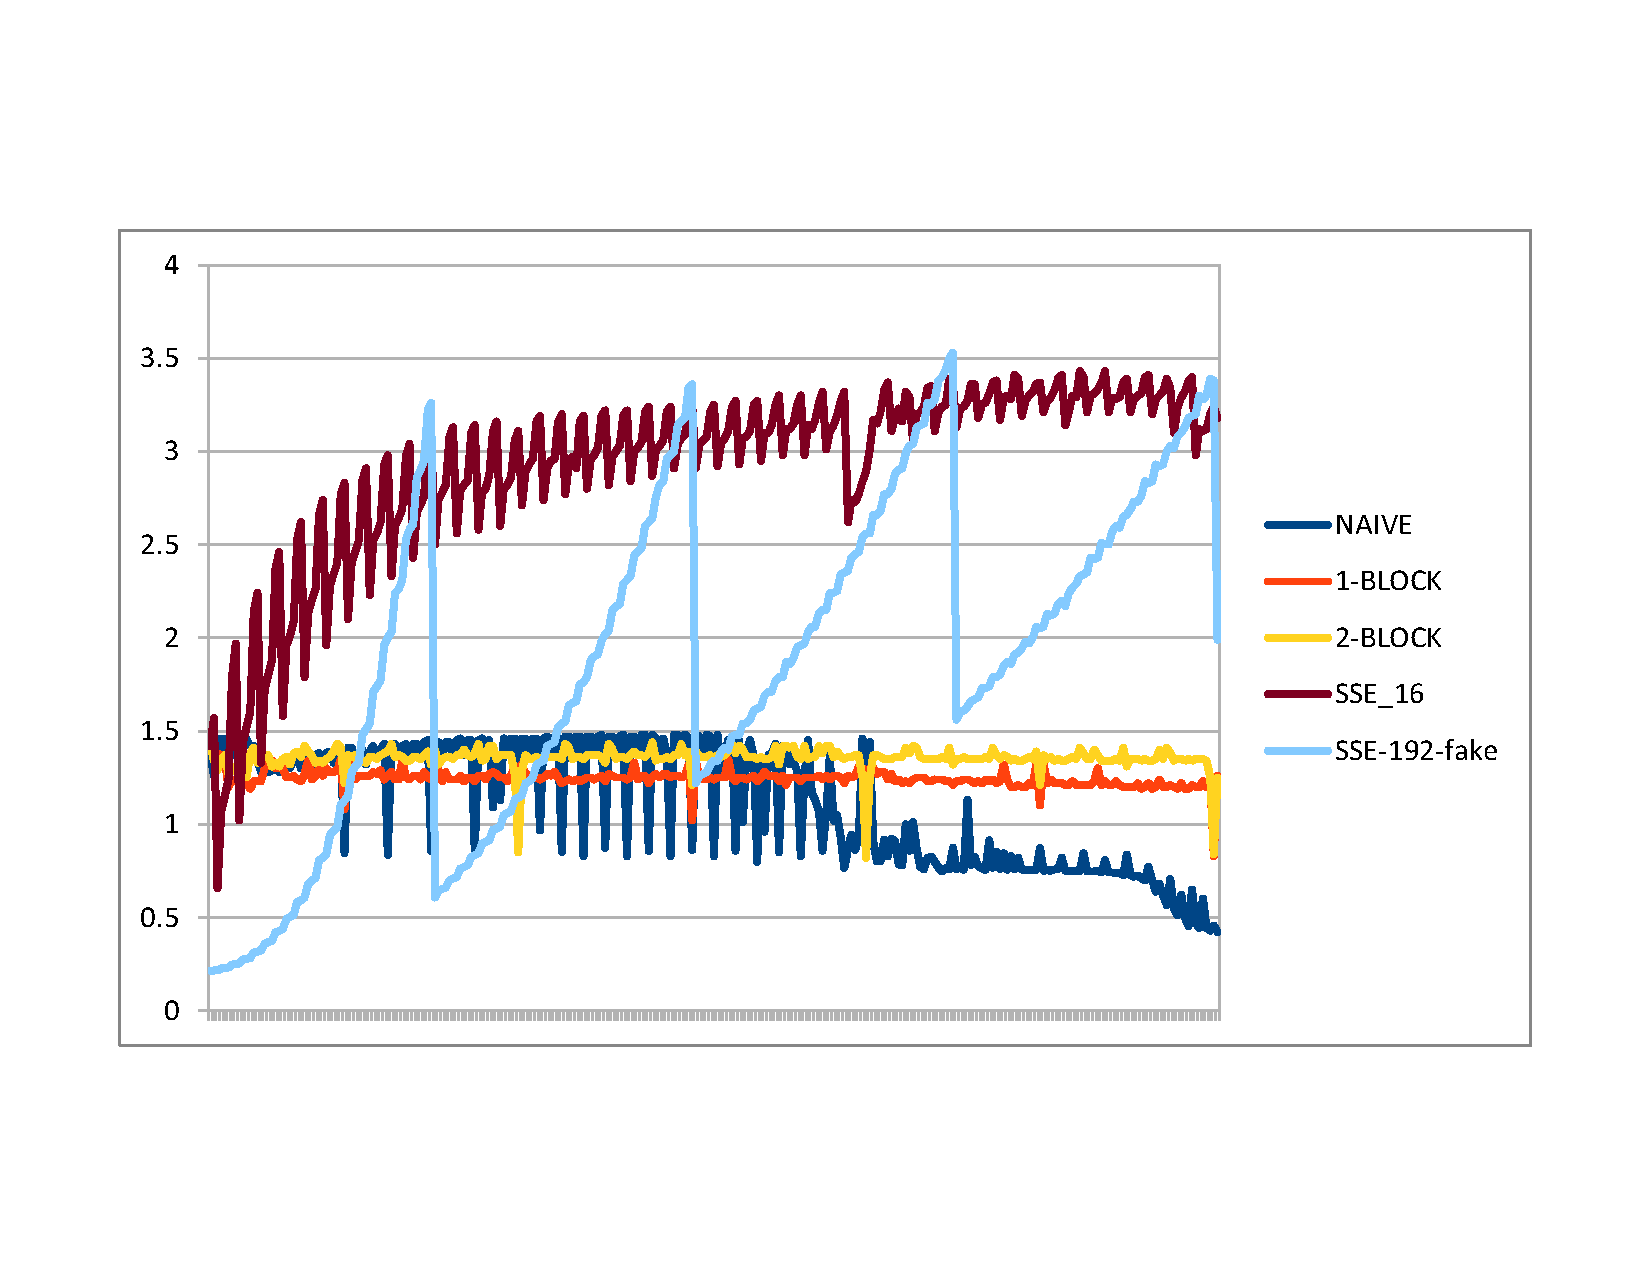
\includegraphics[width=0.7\textwidth]{figures/all_in.pdf}
    \caption{A comparison of all optimizations}
    \label{fig:all_in}
\end{figure}

Figure \ref{fig:all_in} demonstrates some of the optimizations performed and their impact on the overall matrix multiplication performance.

\end{document}
